\documentclass[../notes.tex]{subfiles}

\pagestyle{main}
\renewcommand{\chaptermark}[1]{\markboth{\chaptername\ \thechapter\ (#1)}{}}
\setcounter{chapter}{5}

\begin{document}




\chapter{???}
\section{Module Tools}
\begin{itemize}
    \item \marginnote{2/6:}A fifth week summary has been posted.
    \begin{itemize}
        \item Week 5 content is not in the midterm syllabus.
        \begin{itemize}
            \item In particular, Gauss's Lemma is not on the midterm.
        \end{itemize}
        \item Lecture 5.3 won't even be on the final syllabus.
        \item The techniques are applicable to a variety of problems, though, so it is good to know them.
    \end{itemize}
    \item Today: Modules.
    \begin{itemize}
        \item We depart from commutative rings and return to simple rings with identity to start.
    \end{itemize}
    \item Notation: What kinds of sets different letters denote.
    \begin{itemize}
        \item $A,B$: Rings.
        \item $R$: Commutative ring.
        \item $F,K$: Fields.
        \item $D$: Division ring.
    \end{itemize}
    \item Linear algebra is the study of division rings but only over fields.
    \item Definition of a \textbf{division ring}.
    \begin{itemize}
        \item The only ideals of a division ring are $0,D$, just like with fields.
        \item Linear independence, spanning, basis, etc. all hold in a general division ring; you only need fields for things like JCF.
    \end{itemize}
    \item \textbf{Left $\bm{A}$-module}: An abelian group $(M,+)$ equipped with a binary operation $\cdot:A\times M\to M$ defined by $(a,m)\mapsto am$ (or $a\cdot m$ in the case of potential ambiguity) satisfying the following. \emph{Constraints}\par
    For all $a,b\in A$ and $v,v_1,v_2\in M$\dots
    \begin{enumerate}[label={(\arabic*)}]
        \item $a(v_1+v_2)=av_1+av_2$;
        \item $(a+b)v=av+bv$;
        \item $a(bv)=(ab)v$;
        \item $1_Av=v$.
    \end{enumerate}
    \item We need the last one so that multiplication is nontrivial.
    \item A \textbf{right $\bm{A}$-module} puts the scalar on the right. Will we ever consider these??
    \item Notation: For all $a\in A$, define the function $\rho(a):M\to M$ by $\rho(a)v=av$ for all $v\in M$. \emph{Constraints}
    \begin{enumerate}[label={(\arabic*)}]
        \item $\rho(a)$ is a group homomorphism from $M\to M$.
        \item $\rho(a+b)=\rho(a)+\rho(b)$.
        \item $\rho(a)\rho(b)=\rho(ab)$.
        \item $\rho(1_A)=1_{\End(M)}$
    \end{enumerate}
    \item Conditions 2-4 imply that $\rho:A\to\End(M)$ is a ring homomorphism.
    \begin{itemize}
        \item Recall HW1 Q1.14, which led up to the result that
        \begin{equation*}
            \End(M) = \{f:M\to M\mid f\text{ is a group homomorphism}\}
        \end{equation*}
        is a ring with identity under componentwise addition and composition (i.e., $g\cdot f=g\circ f$).
    \end{itemize}
    \item Going forward, in-class definitions will always match those in the book.
    \begin{itemize}
        \item It's been this way for a while??
    \end{itemize}
    \item Examples.
    \begin{enumerate}
        \item Let $M=A$. Then $\rho(a)b=ab$ for all $a\in A$, $b\in M=A$.
        \item If $M_i$ ($i\in I$ an indexing set) is a (left) $A$-module, then the product $\prod_{i\in I}M_i$ is also an $A$-module.
        \item Denote an element of $\prod_{i\in I}M_i$ by $\prod_{i\in I}m_i$. An arbitrary choice of $m_i\in M_i$ for all $i\in I$ is allowed (do we need the Axiom of Choice??). We define $\cdot$ by
        \begin{equation*}
            a\left( \prod_{i\in I}m_i \right) = \prod_{i\in I}(am_i)
        \end{equation*}
        \item The collection
        \begin{equation*}
            \oplus_{i\in I}M_i = \left\{ \prod_{i\in I}m_i\mid\{i\in I:m_i\neq 0\}\text{ is a finite set} \right\}
        \end{equation*}
        is an $A$-module.
        \begin{itemize}
            \item This is a submodule of something??
            \item Under the same binary operation as Example 3??
        \end{itemize}
        \item In particular, $A^m$ is an $A$-module with $a(b_1,\dots,b_n)=(ab_1,\dots,ab_n)$.
    \end{enumerate}
    \item \textbf{Submodule}: A subgroup $(N,+)$ of $(M,+)$ such that for all $a\in A$ and $\omega\in N$, $a\omega\in N$.
    \item Observation: If $N_1,N_2$ are submodules of $M$, then $N_1+N_2$ and $N_1\cap N_2$ are submodules.
    \item Question (base case): What are the submodules of $A$, itself?
    \begin{itemize}
        \item Left ideals.
    \end{itemize}
    \item \textbf{Module homomorphism}: A function $T:M\to N$ such that $T$ is a homomorphism of abelian groups and commutes with scalar multiplication (i.e., $T(av)=aT(v)$ for all $a\in A$, $v\in M$). In full, we have
    \begin{equation*}
        T(a_1v_1+a_2v_2) = a_1T(v_1)+a_2T(v_2)
    \end{equation*}
    for all $a_1,a_2\in A$ and $v_1,v_2\in M$.
    \item Question: What are all of the module homomorphisms $T:A\to M$?
    \begin{itemize}
        \item If $T(1)=v$, then $T(a\cdot 1)=aT(1)=av$ for all $a\in A$.
        \item For all $v\in M$, there exists a unique $T:A\to M$ such that $T(1)=v$. This is more linear algebra.
    \end{itemize}
    \item Question: What are all linear transformations $T:A^n\to M$?
    \begin{itemize}
        \item Suppose $e_1=(1,0,\dots,0)$, $e_2=(0,1,0,\dots,0)$, etc. Then
        \begin{equation*}
            (a_1,\dots,a_n) = \sum_{i=1}^na_ie_i
        \end{equation*}
        \item Therefore,
        \begin{equation*}
            T(a_1,\dots,a_n) = \sum_{i=1}^na_iTe_i
        \end{equation*}
        \item Take any ordered $n$-tuple of elements in $M$; then given $v_1,\dots,v_n\in M$, there is a unique $A$-module homomorphism $T:A^n\to M$ such that $T(e_i)=v_i$ ($i=1,\dots,n$).
    \end{itemize}
    \item \textbf{Isomorphism} (of $A$-modules): A bijective module homomorphism $T:M\to N$, where $M,N$ are $A$-modules.
    \item It follows that $T^{-1}:N\to M$ is also a homomorphism.
    \item Proposition: Let $N$ be a submodule of $M$. Then the quotient group $M/N$ has a unique structure of an $A$-module such that $\pi:M\to M/N$ (defined with groups) is an $A$-module homomorphism.
    \begin{proof}
        {\color{white}hi}\par
        \underline{Existence}: For all $a\in A$, we have that $\rho(a):M\to M$ take $\rho(a)N\subset N$. It induces $\overline{\rho(a)}:M/N\to M/N$. Take $\overline{\rho(a)}$, which is scalar multiplication by $a$ on $M/N$.
    \end{proof}
    \item FIT: Let $\phi:M\to N$ be a module homomorphism. Then $\ker(\phi)$ is a submodule $M$ and $\im(\phi)$ is a submodule of $N$.
    \begin{figure}[H]
        \centering
        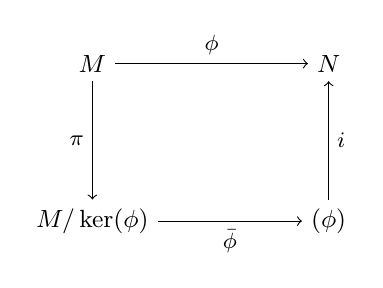
\begin{tikzpicture}[xscale=3,yscale=2]
            \small
            \node (M)  at (0,1) {$M$};
            \node (Mk) at (0,0) {$M/\ker(\phi)$};
            \node (Mi) at (1,0) {$\im(\phi)$};
            \node (N)  at (1,1) {$N$};

            \footnotesize
            \draw [->] (M)  -- node[left] {$\pi$}        (Mk);
            \draw [->] (Mk) -- node[below]{$\bar{\phi}$} (Mi);
            \draw [->] (Mi) -- node[right]{$i$}          (N);
            \draw [->] (M)  -- node[above]{$\phi$}       (N);
        \end{tikzpicture}
        \caption{First isomorphism theorem of modules.}
        \label{fig:FITModule}
    \end{figure}
    \item Example: $A=\Z$ and $M=\Z/(27)$.
    \item Theorem: Let $R$ be a PID. Then every $R$-submodule of $R^n$ is isomorphic to $R^m$ for some $0\leq m\leq n$.
    \item Think in terms of fields! If Nori had been couching all of this in terms of vector spaces, we would all get all of this immediately.
    \item Let $n=1$, $(2)\subsetneq\Z$. Then $m=n$ does not imply $M=R^n$.
    \item Submodules of $R$ are ideals. Thus, in a PID, they're principal ideals.
    \begin{proof}
        Case 1 (base case): Let $n=1$. We know that $M=(b)$ for some $b\in R$. If $b=0$, then we're done. Thus, assume $b\neq 0$. Then $T:R\to(b)$ given by $T(a)=ab$ for all $a\in A$. It follows that $T$ is onto. From the fact that $R$ is an integral domain, we have that $T$ is 1-1.\par
        Case 2 (general case): We induct on $n$. Suppose that $i:R^{n-1}\hookrightarrow R^n$ is given by
        \begin{equation*}
            i(a_1,\dots,a_{n-1}) = (a_1,\dots,a_{n-1},0)
        \end{equation*}
        Let $M$ be a submodule of $R^n$. Then $R^{n-1}\times\{0\}\hookrightarrow R^n$ and $M\cap(R^{n-1}\times\{0\})\cong R^\ell$ for $0\leq\ell\leq n-1$. Suppose that you define the ideal $\pi(a_1,\dots,a_n)=a_n$. Let $\pi(M)=I$. Then you have some ideal $I$. It follows that $\pi:M\to I\subset R$. Let $M'=\ker\phi$. $M/M'\cong I$. At this point, there are only two cases ($a=0$ and $a=M$).
    \end{proof}
    \item Next time: We will wrap up this proof with the following proposition.
    \item Proposition: If $M'$ is a submodule of $M$ and $M/M'\cong R$ as an $R$-module, then $M\cong M'\oplus R$.
\end{itemize}



\section{Office Hours (Nori)}
\begin{itemize}
    \item Is the final cumulative? Will we ever be responsible for the Week 5 material?
    \begin{itemize}
        \item Stuff from Week 5 and this lecture may show up in terms of thought processes you need to go through again, but the exact stuff won't show up. And certainly not on Wednesday's midterm.
        \item The midterm will test who is thinking correctly and who can write proper proofs; there will only be one proof problem, most likely.
        \item Several T/F questions.
        \item If $R[X]$ is a UFD, prove that $R$ is a UFD.
        \item The two Lecture 5.2 methods are important to know (e.g., for the final).
    \end{itemize}
    \item Review questions email?
    \begin{itemize}
        \item Looking at the \emph{fourth week summary} and the problems in there will help you prepare for your midterm.
        \item That may be too strong a statement, but it might be nice.
        \item The gcd of two elements in a PID is just found by looking for a generator. Study this!! Nori wants to put a problem on it.
    \end{itemize}
    \item Lecture 3.1: What is $\bar{X}$ in a quotient ring with a degree 1 or 0 polynomial divisors?
    \begin{itemize}
        \item It is an abrupt and jumpy transition from degree 1 to 0.
        \item For degree $n=0$, we have a natural homomorphism from $\Z/2\Z[X]$ to $\Z[X]/(2)$.
        \item For degree $n\geq 2$ in the ideal, we have a new polynomial that's solvable.
        \item For degree $n=1$, we get dyadics or something like that.
        \item What about $(2X)$? It's kind of in between the $n=1$ and $n=0$ cases. We have an injection
        \begin{equation*}
            \Z[X]/(2X) \hookrightarrow \Z[X]/(2)\times\Z[X]/(X)
            \cong \F_2[X]\times\Z
        \end{equation*}
        \begin{itemize}
            \item We also have a ring homomorphism from $F_2[X]\times\Z\to\F_2\times\F_2$ defined by evaluation in the first slot and then $f(0)$ in the next.
            \item But $(\F_2[X]\times\Z)/(\Z[X]/(2X))\cong\F_2$. This conjugacy only happens as groups, though.
            \item To get down to one element, you can prove that $\Z[X]/(2X)\cong\Delta^{-1}(\F_2)$ where $\Delta$ is the diagonal.
        \end{itemize}
    \end{itemize}
    \item Lecture 4.1: Showing $r\in I$ in this way would not be acceptable in the HW?
    \begin{itemize}
        \item Probably a misstatement.
    \end{itemize}
    \item Lecture 4.2: Incomplete statement on what's all important to prove that something is a UFD.
    \begin{itemize}
        \item It's all important to prove that irreducibles are prime. This is equivalent to $R$ being a UFD.
    \end{itemize}
    \item Lecture 4.2: The whole essay thing and the greatest common divisors being well-defined.
    \begin{itemize}
        \item This is just talking about the algorithm for finding the gcd via factorization.
    \end{itemize}
    \item Section 8.3: Using the Axiom of Choice in the construction of the infinite chain?
    \begin{itemize}
        \item Nori never gives much thought to such matters lol.
        \item You're doing something infinitely many times, but via induction so countably so. Thus, use a countable Axiom of Choice. So it is an Axiom of Choice, but a limited one, too.
    \end{itemize}
    \item Lecture 5.1: Conversely statement.
    \begin{itemize}
        \item Statement (*) provides a "factorization." But for us to know that it actually is a \emph{factorization}, we need to know that each $\pi\in\mathcal{P}(R)$ is, in fact, irreducible. We do that as follows.
        \item Suppose that $\pi=ab$ is a factorization of an irreducible element. By statement (*), write $a=u\pi^{m_0}\pi_1^{m_1}\cdots\pi_h^{m_h}$ and $b=v\pi^{n_0}\pi_1^{n_1}\cdots\pi_h^{n_h}$. It follows that
        \begin{equation*}
            \pi^1\pi_1^0\cdots\pi_h^0 = \pi = ab = \pi^{m_0+n_0}\pi_1^{m_1+n_1}\cdots\pi_h^{m_h+n_h}
        \end{equation*}
        Thus, $m_i+n_i=0$ ($i=1,\dots,h$), so $m_i,n_i=0$ for these $i$. Additionally, $m_0+n_0=1$, so WLOG let $m_0=1$. Then $n_0=0$ and $b$ is a unit. Therefore, $\pi$ is irreducible.
    \end{itemize}
    \item Lecture 5.2: Why do we assume that $a_n\neq 0$?
    \item Lecture 5.2: Clarification on the end of Method 1.
    \begin{itemize}
        \item See Week 5 notes.
        \item Key takeaway: You want to get a bound; it doesn't matter if it's the best possible bound, but a bound on the coefficients of a monic polynomial implies a bound on the roots.
    \end{itemize}
    \item Lecture 5.2: What is going on at the end of Method 2?
    \item Lecture 5.2: What was the thing about reducing polynomials modulo primes?
    \item Lecture 6.1: Will we ever consider right $A$-modules?
    \begin{itemize}
        \item No --- and going forward, \textbf{$\bm{A}$-module} means "left $A$-module."
    \end{itemize}
    \item Lecture 6.1: How long have in-class definitions matched those in the book?
    \begin{itemize}
        \item Practically any book has a different definition of EDs. The book has the weakest definition (i.e., that with the Dedekind-Hasse norm). This definition is basically used nowhere, though.
        \item The \textbf{class group} is a measure of the failure of unique factorizations. This is an example of something that's actually useful.
        \item Rings, ring homomorphisms, etc. But basically stopped in second week.
        \item We need the $\phi(1)=1$ property for instance because otherwise the image of 1 might not act like 1 in the product.
    \end{itemize}
    \item Lecture 6.1: Axiom of Choice needed to pick an element out of each set?
    \item Lecture 6.1: What is the direct product a submodule of?
    \item Lecture 6.1: Is the submodule under the same binary operation as Example?
    \begin{itemize}
        \item The direct sum is a submodule of the product.
    \end{itemize}
\end{itemize}



\section{Office Hours (Ray)}
\begin{itemize}
    \item Do we need proofs for Q5.4?
    \begin{itemize}
        \item No.
    \end{itemize}
    \item What additionally does Q5.1(iii) want us to do?
    \begin{itemize}
        \item You can include a pointer to the previous part and reiterate your proof.
    \end{itemize}
\end{itemize}




\end{document}